\section{Robot Operating System (ROS)}
The Robot Operating System (ROS) is not, like the name may suggest, a full-fledged operating system, but a set of software libraries and tools for the development of robot applications. The open-source robotics middleware comes shipped with capable developer tools, drivers and advanced algorithms. \cite{ros2_documentation}

There are currently two major versions of ROS which are seeing releases, ROS 1 and ROS 2. \cite{ros2_distributions} Beginning with releases after 'Foxy Fitzroy', releases in odd years will be non-LTS (Long Term Support) and will only be supported for 1.5 years, while new releases in even years are going to be long-term supported and will be supported for 5 years. \cite{ros2_releases_and_target_platforms}

The work done in this thesis have been done using the ROS 2 release 'Foxy Fitzroy', released on June 5th, 2020. This release will be supported till the end of May 2023. \cite{ros2_distributions}

\subsection{ROS Graph}
There are 5 main concepts of ROS 2 that make up the ROS (2) graph:
\begin{enumerate}
    \item Nodes
    \item Topics
    \item Services
    \item Parameters
    \item Actions
\end{enumerate}

The ROS graph is a network of ROS 2 elements which processes data simultaneously. The graph encompasses all executables and the connections between them.

\begin{figure}[H]
    \centering
    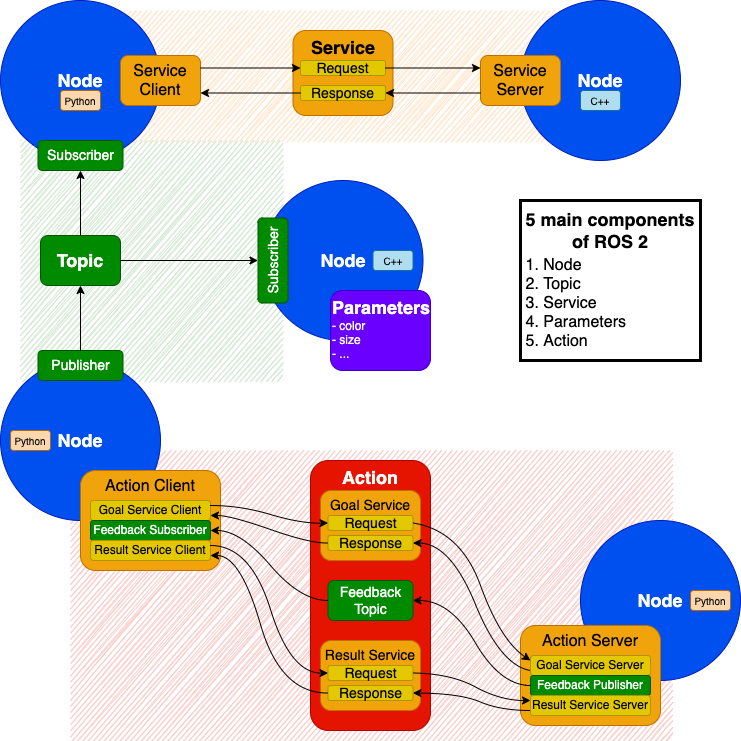
\includegraphics[width=\columnwidth]{ROS2_Main_Concepts.png}
    \caption{The five main concepts of ROS 2 pictured as a network of nodes.}
    \label{fig:ROS 2 main concepts}
\end{figure}

\subsubsection{Nodes}
A node is a fundamental ROS 2 element that serves a single, modular purpose in a robotics system. % https://docs.ros.org/en/foxy/Tutorials/Understanding-ROS2-Nodes.html

\subsubsection{Topics}
 Nodes publish information over topics, which allows any number of other nodes to subscribe to and access that information. % https://docs.ros.org/en/foxy/Tutorials/Topics/Understanding-ROS2-Topics.html

\subsubsection{Services}
Services are based on a call-and-response model, versus topics’ publisher-subscriber model. Services only provide data when they are specifically called by a client. % https://docs.ros.org/en/foxy/Tutorials/Services/Understanding-ROS2-Services.html

\subsubsection{Parameters}
Nodes have parameters to define their default configuration values. %https://docs.ros.org/en/foxy/Tutorials/Parameters/Understanding-ROS2-Parameters.html

\subsubsection{Actions}
Actions are built on topics and services and consist of a goal, feedback, and a result. Actions are like services that allow you to execute long-running tasks, provide regular feedback, and are cancelable. % https://docs.ros.org/en/foxy/Tutorials/Understanding-ROS2-Actions.html

\section{Nvidia Jetson}
\lipsum[1]

\section{Languages and Tools}

\begin{itemize}
    \item ROS 2
    \item Python
    \item LaTeX
    \item Git
    \item VS Code
    \item Azure DevOps
    \item GitHub
    \item other Tools
\end{itemize}